\documentclass{standalone}
\usepackage{tikz}
\usetikzlibrary{patterns, positioning}
\usepackage[sfdefault]{ClearSans} %% option 'sfdefault' activates Clear Sans as the default text font
\usepackage[T1]{fontenc}

\begin{document}
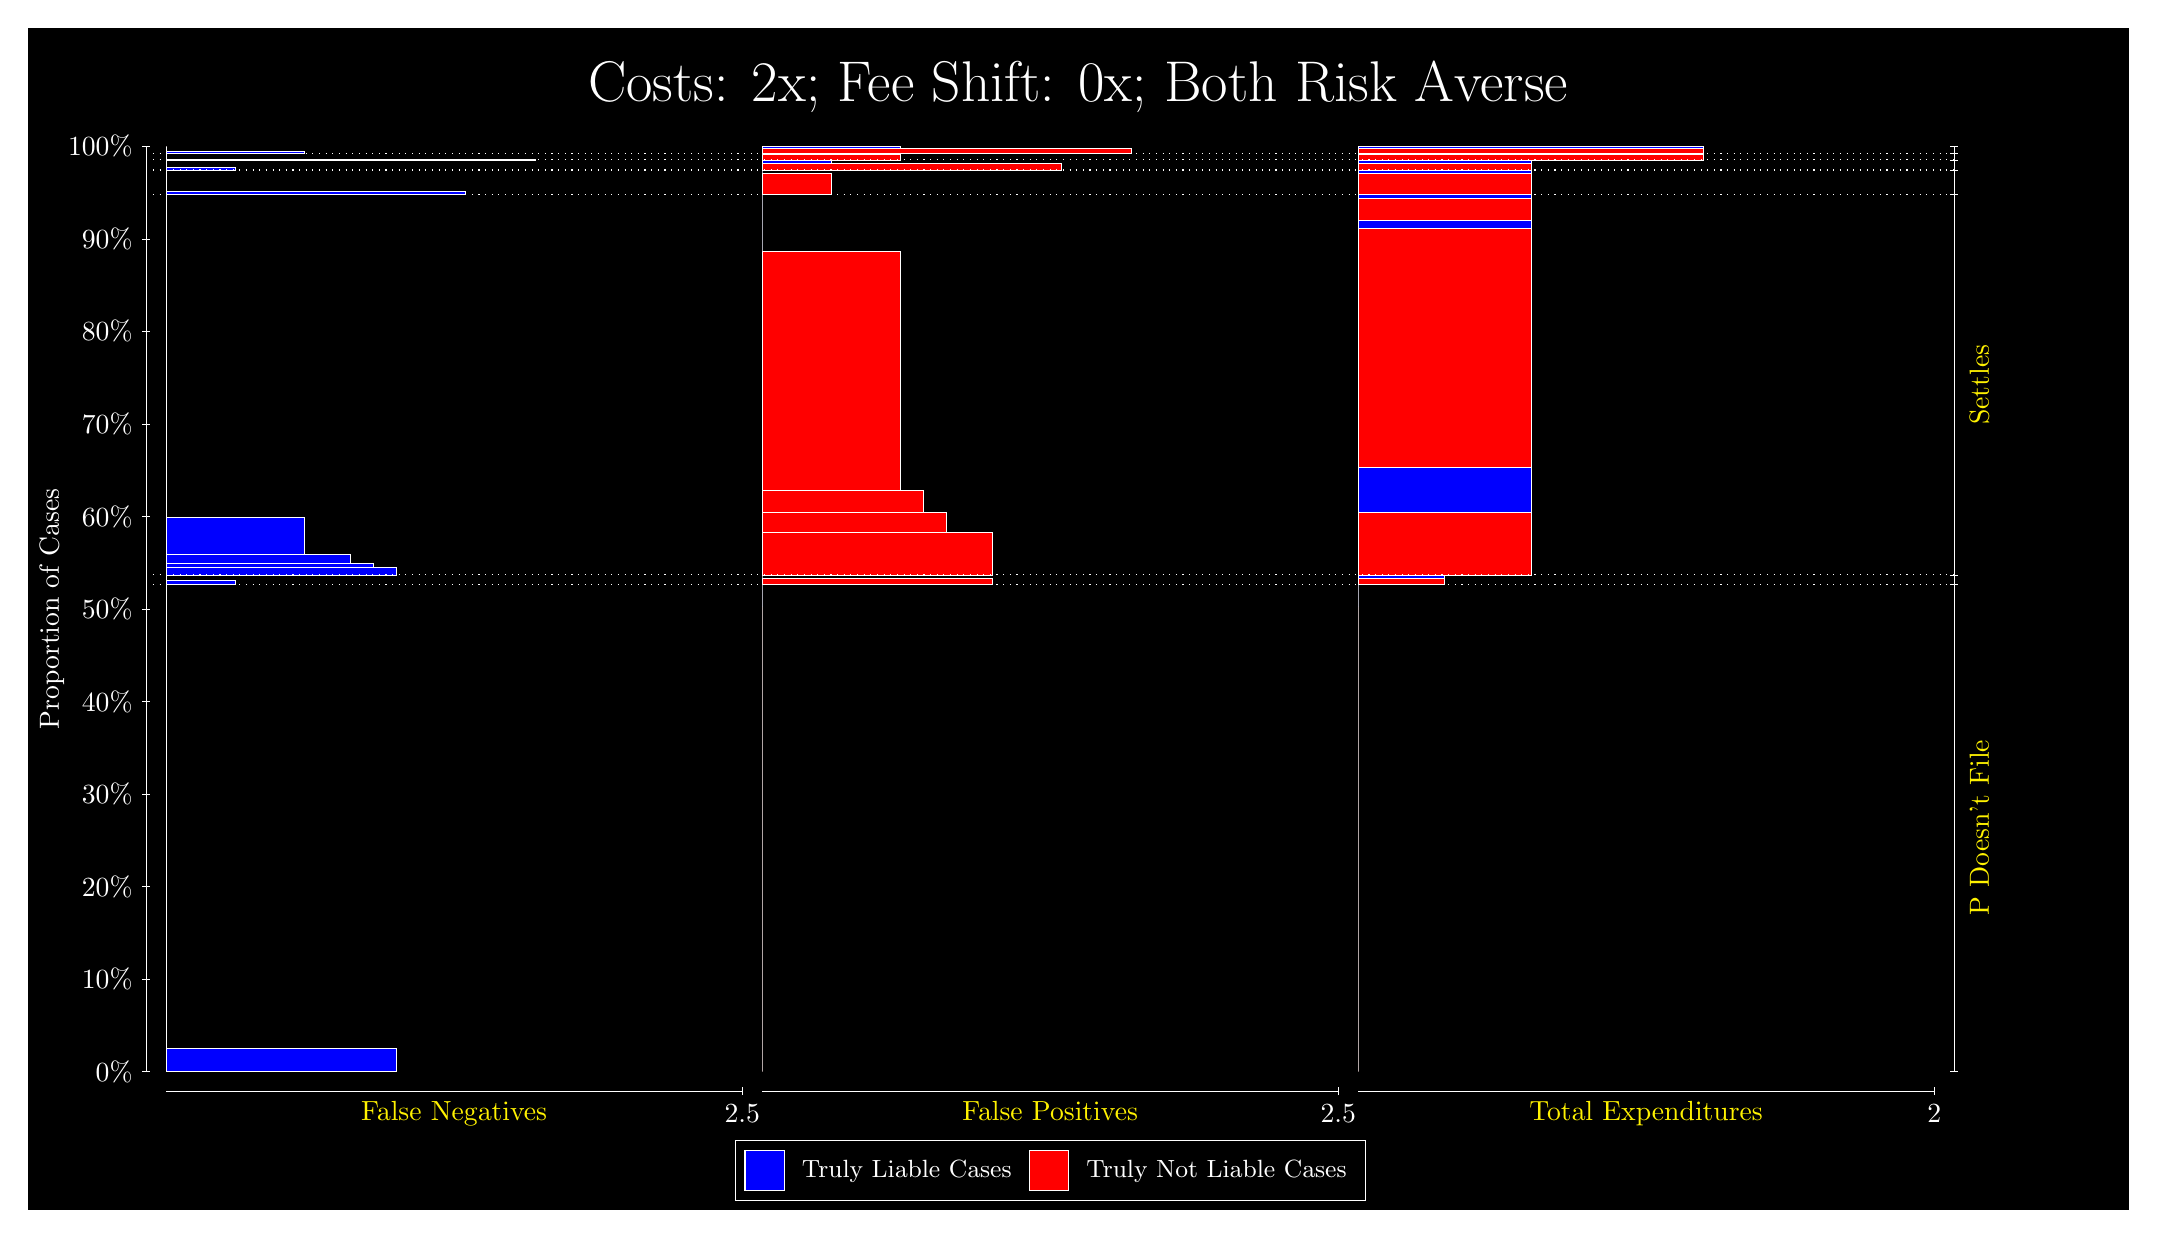
\begin{tikzpicture}
\draw[fill=black] (0,0) rectangle (26.667,15);
\draw[text=white] (0,13.5) rectangle (26.667,15) node[midway] {\huge Costs: 2x; Fee Shift: 0x; Both Risk Averse};
\draw[white, very thin] (1.5,1.75) -- (1.5,13.5);
\node[rotate=90, text=white, anchor=center] at (0.3, 7.625) {Proportion of Cases};
\draw[white, very thin] (1.45,1.75) -- (1.55,1.75);
\node[text=white, anchor=east] at (1.45, 1.75) {0\%};
\draw[white, very thin] (1.45,2.925) -- (1.55,2.925);
\node[text=white, anchor=east] at (1.45, 2.925) {10\%};
\draw[white, very thin] (1.45,4.1) -- (1.55,4.1);
\node[text=white, anchor=east] at (1.45, 4.1) {20\%};
\draw[white, very thin] (1.45,5.275) -- (1.55,5.275);
\node[text=white, anchor=east] at (1.45, 5.275) {30\%};
\draw[white, very thin] (1.45,6.45) -- (1.55,6.45);
\node[text=white, anchor=east] at (1.45, 6.45) {40\%};
\draw[white, very thin] (1.45,7.625) -- (1.55,7.625);
\node[text=white, anchor=east] at (1.45, 7.625) {50\%};
\draw[white, very thin] (1.45,8.8) -- (1.55,8.8);
\node[text=white, anchor=east] at (1.45, 8.8) {60\%};
\draw[white, very thin] (1.45,9.975) -- (1.55,9.975);
\node[text=white, anchor=east] at (1.45, 9.975) {70\%};
\draw[white, very thin] (1.45,11.15) -- (1.55,11.15);
\node[text=white, anchor=east] at (1.45, 11.15) {80\%};
\draw[white, very thin] (1.45,12.325) -- (1.55,12.325);
\node[text=white, anchor=east] at (1.45, 12.325) {90\%};
\draw[white, very thin] (1.45,13.5) -- (1.55,13.5);
\node[text=white, anchor=east] at (1.45, 13.5) {100\%};

\draw[white, very thin] (24.457,1.75) -- (24.457,13.5);
\draw[white, very thin] (24.407,1.75) -- (24.507,1.75);
\node[anchor=west] at (24.407, 1.75) {};
\draw[white, very thin] (24.407,7.9395) -- (24.507,7.9395);
\node[anchor=west] at (24.407, 7.9395) {};
\draw[white, very thin] (24.407,8.0583) -- (24.507,8.0583);
\node[anchor=west] at (24.407, 8.0583) {};
\draw[white, very thin] (24.407,12.888) -- (24.507,12.888);
\node[anchor=west] at (24.407, 12.888) {};
\draw[white, very thin] (24.407,13.199) -- (24.507,13.199);
\node[anchor=west] at (24.407, 13.199) {};
\draw[white, very thin] (24.407,13.329) -- (24.507,13.329);
\node[anchor=west] at (24.407, 13.329) {};
\draw[white, very thin] (24.407,13.407) -- (24.507,13.407);
\node[anchor=west] at (24.407, 13.407) {};
\draw[white, very thin] (24.407,13.5) -- (24.507,13.5);
\node[anchor=west] at (24.407, 13.5) {};

\draw[white, very thin, fill=blue] (1.75,1.75) rectangle (4.6775,2.0392);
\draw[white, very thin, fill=red] (1.75,2.0392) rectangle (1.75,7.9395);
\draw[white, very thin, fill=blue] (1.75,7.9395) rectangle (2.6283,7.9874);
\draw[white, very thin, fill=red] (1.75,7.9874) rectangle (1.75,8.0583);
\draw[white, very thin, fill=blue] (1.75,8.0583) rectangle (4.6775,8.1577);
\draw[white, very thin, fill=blue] (1.75,8.1577) rectangle (4.3848,8.207);
\draw[white, very thin, fill=blue] (1.75,8.207) rectangle (4.092,8.3186);
\draw[white, very thin, fill=blue] (1.75,8.3186) rectangle (3.5065,8.7834);
\draw[white, very thin, fill=red] (1.75,8.7834) rectangle (1.75,12.888);
\draw[white, very thin, fill=blue] (1.75,12.888) rectangle (5.5558,12.927);
\draw[white, very thin, fill=red] (1.75,12.927) rectangle (1.75,13.199);
\draw[white, very thin, fill=blue] (1.75,13.199) rectangle (2.6283,13.238);
\draw[white, very thin, fill=red] (1.75,13.238) rectangle (1.75,13.329);
\draw[white, very thin, fill=blue] (1.75,13.329) rectangle (6.4341,13.336);
\draw[white, very thin, fill=red] (1.75,13.336) rectangle (1.75,13.407);
\draw[white, very thin, fill=blue] (1.75,13.407) rectangle (3.5065,13.434);
\draw[white, very thin, fill=red] (1.75,13.434) rectangle (1.75,13.5);
\draw[white, very thin, fill=red] (9.3189,1.75) rectangle (9.3189,7.6503);
\draw[white, very thin, fill=blue] (9.3189,7.6503) rectangle (9.3189,7.9395);
\draw[white, very thin, fill=red] (9.3189,7.9395) rectangle (12.246,8.0104);
\draw[white, very thin, fill=blue] (9.3189,8.0104) rectangle (9.3189,8.0583);
\draw[white, very thin, fill=red] (9.3189,8.0583) rectangle (12.246,8.6047);
\draw[white, very thin, fill=red] (9.3189,8.6047) rectangle (11.661,8.853);
\draw[white, very thin, fill=red] (9.3189,8.853) rectangle (11.368,9.1312);
\draw[white, very thin, fill=red] (9.3189,9.1312) rectangle (11.075,12.163);
\draw[white, very thin, fill=blue] (9.3189,12.163) rectangle (9.3189,12.888);
\draw[white, very thin, fill=red] (9.3189,12.888) rectangle (10.197,13.16);
\draw[white, very thin, fill=blue] (9.3189,13.16) rectangle (9.3189,13.199);
\draw[white, very thin, fill=red] (9.3189,13.199) rectangle (13.125,13.29);
\draw[white, very thin, fill=blue] (9.3189,13.29) rectangle (10.197,13.329);
\draw[white, very thin, fill=red] (9.3189,13.329) rectangle (11.075,13.399);
\draw[white, very thin, fill=blue] (9.3189,13.399) rectangle (9.3189,13.407);
\draw[white, very thin, fill=red] (9.3189,13.407) rectangle (14.003,13.472);
\draw[white, very thin, fill=blue] (9.3189,13.472) rectangle (11.075,13.5);
\draw[white, very thin, fill=red] (16.888,1.75) rectangle (16.888,7.6503);
\draw[white, very thin, fill=blue] (16.888,7.6503) rectangle (16.888,7.9395);
\draw[white, very thin, fill=red] (16.888,7.9395) rectangle (17.986,8.0104);
\draw[white, very thin, fill=blue] (16.888,8.0104) rectangle (17.986,8.0583);
\draw[white, very thin, fill=red] (16.888,8.0583) rectangle (19.083,8.853);
\draw[white, very thin, fill=blue] (16.888,8.853) rectangle (19.083,9.4294);
\draw[white, very thin, fill=red] (16.888,9.4294) rectangle (19.083,12.461);
\draw[white, very thin, fill=blue] (16.888,12.461) rectangle (19.083,12.561);
\draw[white, very thin, fill=red] (16.888,12.561) rectangle (19.083,12.839);
\draw[white, very thin, fill=blue] (16.888,12.839) rectangle (19.083,12.888);
\draw[white, very thin, fill=red] (16.888,12.888) rectangle (19.083,13.16);
\draw[white, very thin, fill=blue] (16.888,13.16) rectangle (19.083,13.199);
\draw[white, very thin, fill=red] (16.888,13.199) rectangle (19.083,13.29);
\draw[white, very thin, fill=blue] (16.888,13.29) rectangle (19.083,13.329);
\draw[white, very thin, fill=red] (16.888,13.329) rectangle (21.279,13.399);
\draw[white, very thin, fill=blue] (16.888,13.399) rectangle (21.279,13.407);
\draw[white, very thin, fill=red] (16.888,13.407) rectangle (21.279,13.472);
\draw[white, very thin, fill=blue] (16.888,13.472) rectangle (21.279,13.5);
\draw[white, dotted] (1.5,7.9395) -- (24.457,7.9395);
\draw[white, dotted] (1.5,8.0583) -- (24.457,8.0583);
\draw[white, dotted] (1.5,12.888) -- (24.457,12.888);
\draw[white, dotted] (1.5,13.199) -- (24.457,13.199);
\draw[white, dotted] (1.5,13.329) -- (24.457,13.329);
\draw[white, dotted] (1.5,13.407) -- (24.457,13.407);
\draw[white, very thin] (1.75,1.5) -- (9.0689,1.5);
\node[text=yellow, anchor=north] at (5.4094, 1.5) {False Negatives};
\draw[white, very thin] (9.0689,1.45) -- (9.0689,1.55);
\node[text=white, anchor=north] at (9.0689, 1.45) {2.5};

\draw[white, very thin] (9.3189,1.5) -- (16.638,1.5);
\node[text=yellow, anchor=north] at (12.978, 1.5) {False Positives};
\draw[white, very thin] (16.638,1.45) -- (16.638,1.55);
\node[text=white, anchor=north] at (16.638, 1.45) {2.5};

\draw[white, very thin] (16.888,1.5) -- (24.207,1.5);
\node[text=yellow, anchor=north] at (20.547, 1.5) {Total Expenditures};
\draw[white, very thin] (24.207,1.45) -- (24.207,1.55);
\node[text=white, anchor=north] at (24.207, 1.45) {2};

\node[text=yellow, centered, rotate=90] at (24.777, 4.8447) {P Doesn't File};

\node[text=yellow, centered, rotate=90] at (24.777, 10.473) {Settles};





\draw (12.978300999999998,1.5) node[draw=none] (baseCoordinate) {};
\begin{scope}[align=center]
        \matrix[scale=0.5, draw=white, below=0.5cm of baseCoordinate, nodes={draw}, column sep=0.1cm]{
            \node[rectangle, draw, minimum width=0.5cm, minimum height=0.5cm, fill=blue] {}; &
            \node[draw=none, font=\small, text=white] (B) {Truly Liable Cases}; &
            \node[rectangle, draw, minimum width=0.5cm, minimum height=0.5cm, fill=red] {}; &
            \node[draw=none, font=\small, text=white] (B) {Truly Not Liable Cases}; \\
            };
\end{scope}

\end{tikzpicture}
\end{document}